% % % % % % % % % % % % % % % % % % % % % % % % %
%  
%  Figure captions for the LTP paper
%
%  Copyright (c) 2017 - EMBL
%
%  File author(s):
%    Dénes Türei (denes@ebi.ac.uk)
%
%  This file is not intended for public use.
%  Please do not use and do not redistribute it.
%  
%  Website: http://www.ebi.ac.uk/~denes
%
%  Tested with XeTeX, Version 3.14159265-2.6-0.99992
%  (TeX Live 2015/Arch Linux)
%
%  
% % % % % % % % % % % % % % % % % % % % % % % % %
%
% I already put many stuff in the headings.
% The actual text starts somewhere after line 200
%
% Comments implemented with `todonote` package.
% Simply place \todo{...comment...} anywhere inline.
% After second recompilation these will be properly
% placed in the PDF. To suppress them add the `final`
% option to documentclass.
%
% % % % % % % % % % % % % % % % % % % % % % % % %

\documentclass[11pt, a4paper]{article}
\usepackage[no-math]{fontspec}
\usepackage{xunicode}
\usepackage{polyglossia}
\setdefaultlanguage{english}
\usepackage{xltxtra}
\usepackage{fullpage}
%\usepackage{lineno}
\usepackage{setspace}
\usepackage{hyperref}
\hypersetup{colorlinks=true, linkcolor=emblpetrol, citecolor=emblpetrol, filecolor=emblpetrol, urlcolor=emblpetrol,
    pdftitle='LTP paper figure layouts and captions',
    pdfauthor={Dénes Türei},
    pdfborder={0, 0, 0},
    breaklinks=true, pdfpagemode=UseNone, pageanchor=true, pdfpagemode=UseOutlines,
    hypertexnames=true, pdfhighlight=/O, pdfstartpage=1, pdfstartview=FitV, linktocpage=false,
    pdfsubject={LTP paper figure layouts and captions},
    pdfkeywords={
        LTP,
        lipid transfer protein,
        lipid,
        mass spectrometry
    },
    pdfcreator={XeTeX}}
%\usepackage{doi}
\usepackage{csquotes}
%\usepackage[cm]{fullpage}
\usepackage{microtype}
%\usepackage{xkvltxp}
\usepackage{graphicx}
%\usepackage{titling}
% suppress section numbers
\usepackage{titlesec}

% figures
\usepackage{caption}
\usepackage{subcaption}
%\usepackage{subfig}

% floats
\usepackage{rotating}
\usepackage{newfloat}
\usepackage{morefloats}
\usepackage{chngcntr}
\usepackage{wrapfig}
%\usepackage{ccaption}
%\usepackage[CaptionAfterwards]{fltpage}

% tables
\usepackage{tabularx}
\usepackage{booktabs}
\usepackage{array}

\usepackage{cleveref}
\usepackage{xcolor}

\usepackage{amsmath}
\usepackage{amssymb}
\usepackage{amsfonts}
\usepackage{mathtools}
\usepackage{units}
\usepackage{textcomp}
\usepackage{bm}

\usepackage{tikz}
%\usepackage[obeyFinal, textsize=tiny, backgroundcolor=emblzircon,
%textwidth=3cm, bordercolor=white, linecolor=emblpetrol]{todonotes}

%\usepackage[flushmargin,hang,multiple]{footmisc}
%\renewcommand{\footnotelayout}{\protect\raggedright\textsf}

% matrix bold capitals
\newcommand\mat[1]{\bm{#1}}

\usepackage{etoolbox}
\patchcmd{\thanks}{#1}{\protect\raggedright#1}{}{}


\newfontface{\sentinel}[Path=fonts/]{Sentinel-Book.otf}
\newfontface{\sentinelitalic}[Path=fonts/]{Sentinel-BookItalic.otf}
\newfontface{\sentinelbold}[Path=fonts/]{Sentinel-Bold.otf}
\newfontface{\sentinelsemibold}[Path=fonts/]{Sentinel-Semibold.otf}
\newfontface{\helveticalight}[Path=fonts/]{HelveticaNeueLTStd-Lt.otf}

\setmainfont{Sentinel-Book.otf}[Path=fonts/, BoldFont=Sentinel-Semibold.otf, ItalicFont=Sentinel-BookItalic.otf]
\setsansfont{HelveticaNeueLTStd-LtCn.otf}[Path=fonts/, BoldFont=HelveticaNeueLTStd-MdCn.otf]

% kerning of this font is not perfect...
\spaceskip=1.5\fontdimen2\font plus 1.5\fontdimen3\font
minus 1.5\fontdimen4\font

% now seems to be standard in english typography:
\frenchspacing

% these have been removed as we prepare the final version:
%\onehalfspace
%
%\linenumbers

% colors
\definecolor{emblpetrol}{RGB}{68, 119, 170}
\definecolor{emblgreen}{RGB}{17, 119, 119}

%\definecolor{embltwilight}{RGB}{239, 244, 233}
%\definecolor{emblzircon}{RGB}{228, 236, 236}
%\definecolor{emblyellow}{RGB}{250, 183, 0}
%\definecolor{emblred}{RGB}{227, 62, 62}
%\definecolor{emblgray1}{gray}{0.875}
%\definecolor{emblgray8}{gray}{0.125}
%\definecolor{emblgray75}{gray}{0.25}

% footnote counters
\newcounter{savecntr}% Save footnote counter
\newcounter{restorecntr}% Restore footnote counter

\title{LTP paper figure layouts and captions}
\date{\today}


   
% supplementary figure numbering
\DeclareFloatingEnvironment[name={Supplementary Figure}]{csuppfigure}
\DeclareFloatingEnvironment[name={Figure}]{suppfigure}

\DeclareFloatingEnvironment[name={Table}]{supptable}
\DeclareFloatingEnvironment[name={Supplementary Table}]{csupptable}


% % % % % % % % % % % % % % % % % % % % % % % % % % % % % % % % % % %

\definecolor{glacier}{RGB}{134, 173, 194}
\definecolor{spindle}{RGB}{186, 189, 213}
\definecolor{kobi}{RGB}{186, 189, 213}
\definecolor{chathams}{RGB}{157, 203, 162}
\definecolor{medgreen}{RGB}{17,119,68}

% this was to hihlight new additions:
% \newcommand{\new}[1]{{\color{medgreen}#1}}
\newcommand{\new}[1]{#1}

% subfigure captions

\captionsetup[subfigure]{position=t, labelfont={sf, bf}, textfont=normalfont, labelformat=simple, singlelinecheck=off, justification=raggedright}

\captionsetup[table]{position=t, labelfont=normalfont, textfont=normalfont, singlelinecheck=off, justification=raggedright}
\captionsetup[supptable]{position=t, labelfont=normalfont, textfont=normalfont, singlelinecheck=off, justification=raggedright}

\setlength{\skip\footins}{2\baselineskip}
    
    % % % % % % % % % % % % % % % % % % % % % % % % % % % % % % % % % % %
    % % % % % % % % % % % % % % % % % % % % % % % % % % % % % % % % % % %
    
    \begin{document}
    
    \section*{Main Text Figures}
    
    \begin{figure}[!h]
           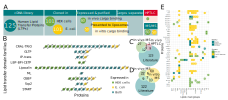
\includegraphics[width=\textwidth]{fig1.pdf}
       \caption{\label{fig:fig1}\textbf{High-throughput screening of human lipid transfer protein cargoes.} \textbullet\ \textbf{(A) Our screening space covers more than half of all human LTPs.} We formerly collected from the literature a list of 125 human proteins capable to carry hydrophobic metabolites through aqueous phases inside their dedicated binding pocket (Chiapparino 2016). We constructed a cDNA library of the 125 lipid transfer proteins (LTPs). We successfully cloned 101 of them in HEK 293T cells and ?? (\new{I don't know the number}) in \textit{E. coli.}} 60 LTPs we were able to purify from HEK cells and 50 from \textit{E. coli.} In HEK cells we assumed the proteins bound their ligands \textit{in vivo}, while the \textit{E. coli} expressed proteins we exposed to bovine brain whole lipid extract liposomes to achieve an \textit{in vitro} ligand binding. After we separated the hydrophobic ligands and we analyzed 13 of the \textit{in vivo} produced by high-performance thin-layer chromatography (HPTLC) and all of them by LC/MS/MS using both positive and negative ion mode. \textbf{(B) The two screenings increase the coverage and gives opportunity for cross-confirmation.} We could produce 73 proteins in total, 23 only in HEK cells, 13 only in \textit{E. coli} while 37 in both. The lipid transfer domains of these proteins belong to 9 domain families. \textbf{(C-D) Overlaps between our screenings among each other and the prior knowledge from the literature (Chiapparino 2016).} Number of protein-lipid relationships at the level of main lipid categories (e.g. phosphatidylcholine). \textbf{(E) Results of our MS screening at the level of main lipid categories.} Novel relationships are marked with dot.
    \end{figure}
   
    % % % % % % % % % % % % % % % % % % % % % %
    \clearpage
    \setcounter{figure}{0}
    
    \begin{figure}[p]
        \includegraphics[width=\textwidth]{fig1v2.pdf}
    \end{figure}
    
    \subsection*{Alternative layout for Figure 1}
    \captionof{figure}{\label{fig:fig1v2}\textit{(Opposite page)} \textbf{High-throughput screening of human lipid transfer protein cargoes.} \textbullet\ \textbf{(A) Our screening space covers more than half of all human LTPs.} We formerly collected from the literature a list of 125 human proteins capable to carry hydrophobic metabolites through aqueous phases inside their dedicated binding pocket (Chiapparino 2016). We constructed a cDNA library of the 125 lipid transfer proteins (LTPs). We successfully cloned 101 of them in HEK 293T cells and ?? (\new{I don't know the number}) in \textit{E. coli.}} 60 LTPs we were able to purify from HEK cells and 50 from \textit{E. coli.} In HEK cells we assumed the proteins bound their ligands \textit{in vivo}, while the \textit{E. coli} expressed proteins we exposed to bovine brain whole lipid extract liposomes to achieve an \textit{in vitro} ligand binding. After we separated the hydrophobic ligands and we analyzed 13 of the \textit{in vivo} produced by high-performance thin-layer chromatography (HPTLC) and all of them by LC/MS/MS using both positive and negative ion mode. \textbf{(B-C) The two screenings increase the coverage and gives opportunity for cross-confirmation.} Overlaps between our screenings among each other and the prior knowledge from the literature (Chiapparino 2016). Number of protein-lipid relationships at the level of main lipid categories (e.g. phosphatidylcholine). \textbf{(D) Results of our MS screening at the level of main lipid categories.} Novel relationships are marked with dot.
    
    % % % % % % % % % % % % % % % % % % % % % %
    \clearpage
    \stepcounter{figure}
    
    \begin{figure}[p]
        \includegraphics[width=\textwidth]{fig3.pdf}
    \end{figure}


        \captionof{figure}{\textit{(Opposite page)} \textbf{From raw MS data to a landscape of protein-lipid cargo interactions. \textbullet\ (A) Selection and identification of MS detected features.} The graph in the middle shows the number of features at each stage of the selection. Each line represents one protein in one ion mode. (1) The identical \nicefrac{m}{z} values within and across fractions have been assembled using the PEAKS software. This resulted 10-40 thousands of features for each protein and ion mode. (2) We selected the features which have been seen along multiple scans (peak quality) and their intensity in the protein containing fractions was at least twice higher than in the void fractions (peak size) and also had single charge and retention time over 1 min. (3) We applied semi-quantitative criteria to select the features which show intensity pattern similar to the protein concentration across fractions. The inset illustrates the concentration of FABP1 protein (green columns) and the MS feature intensities showing similar pattern (blue and red, negative and positive ion modes, respectively) in the \textit{in vitro} screening. To identify the features we looked up the the MS1 masses in metabolic databases (SwissLipids and LipidMaps) and analyzed the MS2 scans comparing them to our own standards and the literature. (4) We manually checked the identification of the features fulfilling all the selection criteria. We classified based on their identification level into classes defined in Table X. Finally we considered in our final result all unambiguously identified features from either of the screenings in case these were supported by MS2 and those lacking MS2 data but confirmed by both screenings (Supplementary Figure \ref*{fig:roc}.). \textbf{(B) Protein-lipid relationships in the MS screenings.} The outer circle represents the proteins and large categories of lipids (e.g. glycerophospholipids, GLP). Proteins are ordered by clustering their lipid relationships and colored by their involvement in the screenings. The inner circle is segmented and colored by the main categories of lipids. The two inner bands are heatmaps of intensities, positive and negative ion modes are shown in red and blue, respectively. Links represent individual protein-lipid relationships (e.g. STARD10-PC(16:1/18:0)) and colored according to main lipid categories. \label{fig:fig3}}

    \clearpage
   
    % % % % % % % % % % % % % % % % % % % % % % % % % % % % % % % % % % % % % % % %
    % % % % %                                                       % % % % % % % %
    % % % % %  S U P P L E M E N T A R Y    I N F O R M A T I O N   % % % % % % % %
    % % % % %                                                       % % % % % % % %
    % % % % % % % % % % % % % % % % % % % % % % % % % % % % % % % % % % % % % % % %
    
    %\resetlinenumber
    \setcounter{page}{1}
    \renewcommand*{\thepage}{S\arabic{page}}
    \renewcommand{\theequation}{S\arabic{equation}}
    \renewcommand{\thesuppfigure}{S\arabic{suppfigure}}
    \renewcommand{\thesupptable}{S\arabic{supptable}}
    
    % % % % % %
    \begingroup
    % % % % % %
    
    \titleformat{\section}%
        [hang]% <shape>
        {\normalfont\bfseries\Large}% <format>
        {}% <label>
        {0pt}% <sep>
        {}% <before code>
    
    \newcounter{ssubsection}
    \newcounter{csubsection}
    \setcounter{ssubsection}{0}
    \setcounter{csubsection}{0}
    \renewcommand{\thesubsection}{Sup. Results S\arabic{subsection}}
    \renewcommand{\thesection}{}% Remove section references...
    \renewcommand{\thefootnote}{\fnsymbol{footnote}}
    \renewcommand{\thefigure}{S\arabic{figure}}
    \renewcommand{\thetable}{S\arabic{figure}}
    \setcounter{footnote}{0}
    
    \section*{Supplementary Figures}
    
    \begin{suppfigure}[!h]
        \includegraphics[width=.75\textwidth]{ms_feature_counts.pdf}
        %           \vspace*{-9\baselineskip}
        \caption{\textbf{Number of features across stages of selection.} One line represent one protein in one ion mode and screening. Screenings and ion modes presented on subplots.\label{fig:numf}}
    \end{suppfigure}
    
    \begin{suppfigure}[!h]
        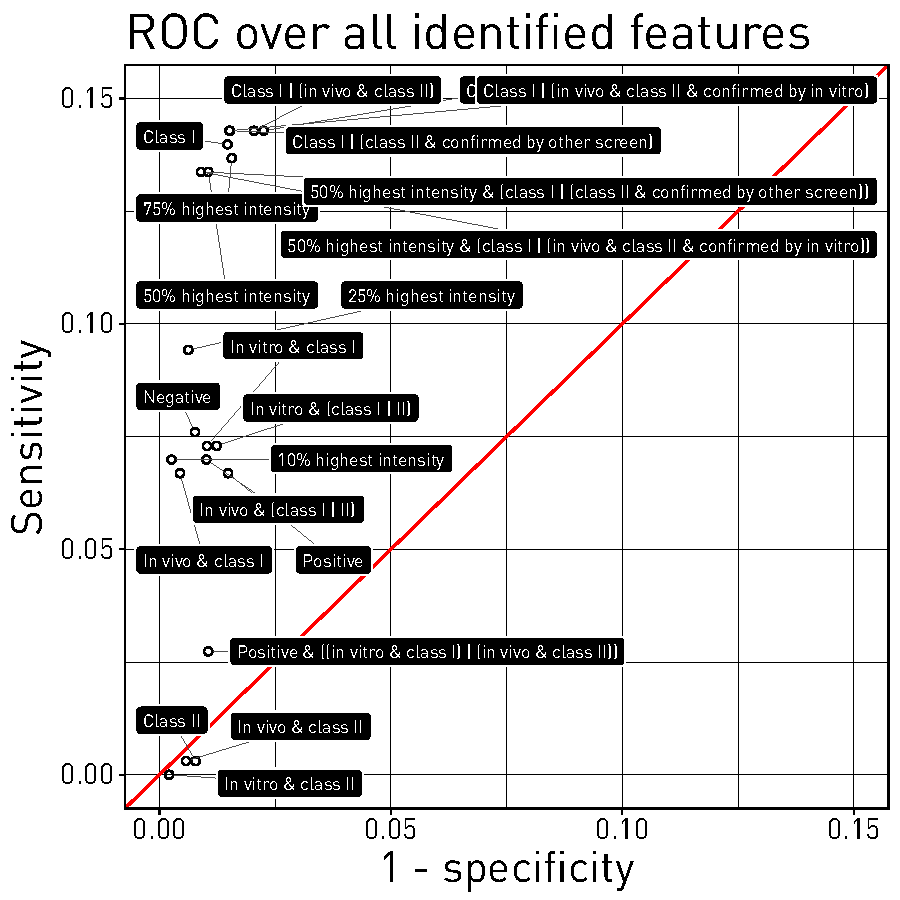
\includegraphics[width=.6\textwidth]{roc_classes_full.pdf}
        %           \vspace*{-9\baselineskip}
        \caption{\textbf{Defining the final results with benchmarking against the literature.} We evaluated the relevance of various conditions by measuring the proportion of literature known relationships recovered. Each point represent one set of conditions and shows the sensitivity and specificity considering the literature as golden standard. We investigated the relevance of intensity, ion mode, the \textit{in vivo} and \textit{in vitro} experimental system and the identification classes. As the ``Class I from either of the screenings and Class II cross-confirmed between the screenings'' shows the highest specificity and sensitivity, we decided to present these features as final results.\label{fig:roc}}
    \end{suppfigure}

\end{document}